\begin{scanpage}{0204}{186}
In \S\ 28 and 29, we noted that current waves are reflected from the ends of a finite length conductor the same as from the end of a semi-infinite conductor, and that the diffraction of these waves at each end takes place in the same way as at the end of a semi-infinite conductor. Therefore, the primary edge waves may be found from the problem of scattering of a plane wave by the semi-infinite conductor $(z_1,\infty)$ and the conductor $(-\infty,z_2)$. The sum of such waves gives the primary diffraction field
\[E_\vartheta^{(1)}=H_\varphi^{(1)}=-E\frac{e^{ikR}}{kR}\cdot F^{(1)}(\vartheta,\vartheta_0),\tag{30.03}\]
where
\[
\begin{aligned}
F^{(1)}(\vartheta,\vartheta_0)={}&\frac{i}{2}\frac{\ctg\dfrac\vartheta2\ctg\dfrac{\vartheta_0}2}{(\cos\vartheta+\cos\vartheta_0)\Phi(-k\cos\vartheta,-k\cos\vartheta_0)}e^{-ikz_1(\cos\vartheta+\cos\vartheta_0)}\\
&-\frac{i}{2}\frac{\tg\dfrac\vartheta2\tg\dfrac{\vartheta_0}2}{(\cos\vartheta+\cos\vartheta_0)\Phi(k\cos\vartheta,k\cos\vartheta_0)}e^{-ikz_2(\cos\vartheta+\cos\vartheta_0)}.
\end{aligned}\tag{30.04}
\]
\par\medskip\noindent\begin{minipage}[t]{.45\linewidth}\vspace{0pt}
\centering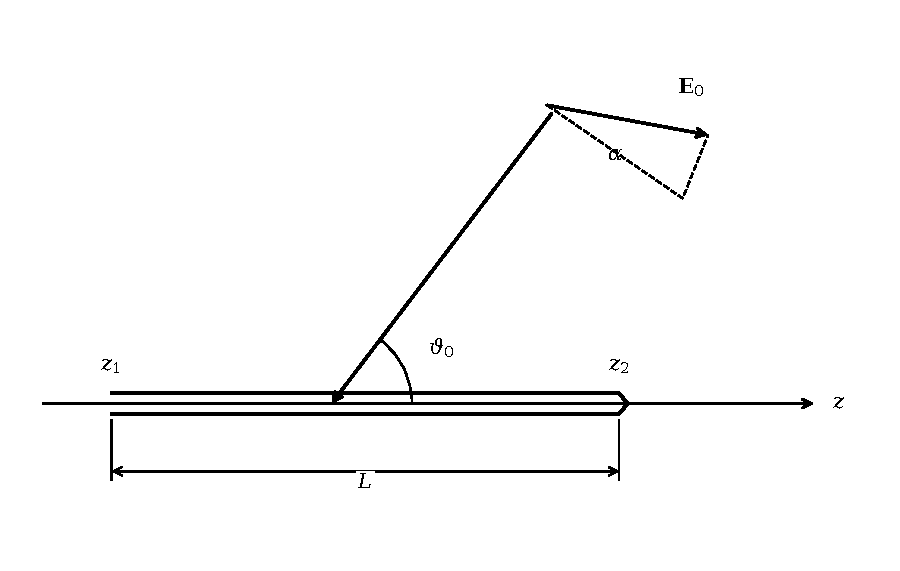
\includegraphics[width=.75\linewidth]{images/recreated/r-0204-fig73.pdf}\par
\small Figure 73. The incidence of a plane wave on a thin cylindrical conductor; $\vartheta_0$ is the incident angle.
\end{minipage}\hfill\begin{minipage}[t]{.51\linewidth}\vspace{0pt}
The function $\Phi(w,w_0)$ may be calculated by means of the rigorous solution to the problem of a semi-infinite vibrator (see [82] \S\ 3 and [83] \S\ 4), and in this case, it satisfies the relationship
\end{minipage}
\[
\left.\begin{aligned}
\Phi(w,w_0)\Phi(-w,-w_0)&=\ln\frac{2i}{\gamma va}\ln\frac{2i}{\gamma v_0a},\\
v=\sqrt{k^2-w^2},\quad v_0&=\sqrt{k^2-w_0^2}.
\end{aligned}\right\}\tag{30.05}
\]
However, henceforth it will not be necessary to have the rigorous expression for the function $\Phi$. Let us note that Equations (30.03) and (30.04) are similar to Expressions (6.13) for a strip. These latter expressions do not take into account secondary diffraction.
\end{scanpage}
